Afin de comprendre comment se déroule la création de la partie nous avons réaliser deux diagrammes.

Le premier, un diagramme de cas d'utilisation nous permet d'illustrer les actions que le joueur est autorisé à faire dans le fonctionnement normal du jeu.
\begin{figure}[!h]
\centering
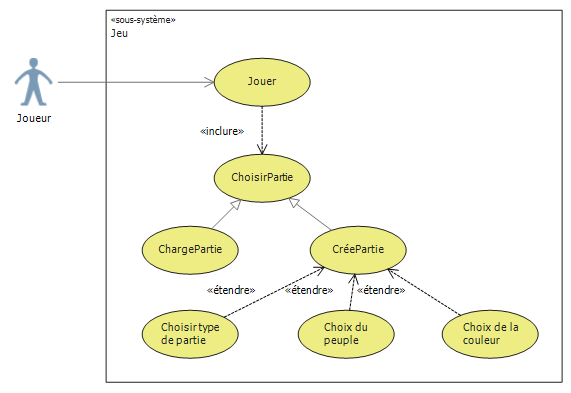
\includegraphics[width=\textwidth]{Parties/Images/cdu_CreationPartie.png}
\caption{Diagramme de cas d'utilisation : création d'une partie}
\label{fig:cdu_CreationPartie}
\end{figure}
